% --------------------------------------------------------------
% This is all preamble stuff that you don't have to worry about.
% Head down to where it says "Start here"
% --------------------------------------------------------------
 
\documentclass[12pt]{article}
\usepackage[margin=1in]{geometry} 
\usepackage{amsmath,amsthm,amssymb}
\usepackage{xcolor}
\usepackage{hyperref}
\hypersetup{
    colorlinks,
    citecolor=black,
    filecolor=black,
    linkcolor=black,
    urlcolor=blue
}
\newcommand{\code}{\texttt}
\setcounter{secnumdepth}{0}
\usepackage{graphicx}
\usepackage{epstopdf}
\usepackage{hyperref}
\epstopdfsetup{outdir=./}
\begin{document}
\title{\textbf{Compilers-II  (CS3423)}\\~\\Mini Assignment - I\\~\\An Introduction to the LLVM Infrastructure, AST, IR and Compiler Options}
\author{Sagar Jain\\CS17BTECH11034}
\maketitle
\begin{normalsize}
\tableofcontents
\end{normalsize}
\newpage
\section{Clang AST}
Clang is essentially a library that allows us to convert a  C program into an Abstract Syntax Tree and then manipulte the tree in some ways.
After viewing the ast for several non-trivial programs the following are a few observations:
\begin{enumerate}
\item The ast for any program can be printed using:\\ \code{clang -Xclang -ast-dump -fsyntax-only <filename>}. Here \code{Xclang} option is used to pass the arguments to the clang compiler, \code{fsyntax-only} is used so that no object code is generated and \code{ast-dump} is used to print the abstract syntax tree.
\item The dump begins with a bunch of \code{TypedefDecl} nodes followed by the ast for the user code.
\item We can use the option \code{ast-list} to get all a list of all the \textit{Declaration} nodes, this is an alternative option to look at the contents of the ast.
\item The \code{ast-view} option lets us look at an the entire ast graphically and is very easy to understand compared to the dump.Internally it creates a dot file which can be viewed by any dot file renderer. Example:
\begin{center}
\includegraphics[scale=0.6]{clangExamples/graph.eps}
\end{center}
\item \texttt{ast-print} option allows us to pretty print the ast with as much resemblence to the orignal code as possible.
\item We can also use clang-check to filter and print only the ast of a subset of the Declaration nodes:\\
\code{clang-check <filename> -ast-dump -ast-dump-filter=main --}
\end{enumerate}
\subsection{Observations about the AST structure}
\begin{itemize}
\item In the tree that clang creates, every node is an instance of one of the two classes: \textbf{Decl} or \textbf{Stmt} class. Nodes usually have a name followed by a type. For example, the main function begins with a \code{FunctionDecl} node which would have a name \textit{main} and a type(say \code{int} or \code{void}).
\item Functions start with \code{FunctionDecl} node which has the function name and type along with it. These are always followed by the \code{ParamVarDecl} nodes which have information about the function parameters and their types.
\item Most of the nodes in the body of the functions belongs to the Stmt class in the form of either of the following:
\begin{itemize}
\item CompoundStmt
\item DeclStmt
\item ImplicitCastExpr
\item CallExpr
\item ReturnStmt
\item Literals, etc.
\end{itemize}
\item Nodes like \code{ForStmt} have multiple children (5 for ForStmt) which are themselves nodes of different kind.
\item Nodes like \code{IntegerLiteral} contain the value of the node as well along with the type.
\item A point to note would be that the nodes themselves do not contain too much information but using the nodes we can get information from the AST context where most of the information is stored.
\end{itemize}
\newpage
\section{Clang AST Traversal}
The observations made about the AST traversal follows from this \href{http://clang.llvm.org/docs/RAVFrontendAction.html}{tutorial}.
\subsection{FrontendAction}
The class ASTFrontendAction is provided to us to be able to interact with the ast while compilation. We must create a class which inherits from FrontendAction to be able to execute user specific actions on the ast. We must implement a virtual method \code{CreateASTConsumer} in this class which returns a type of \code{std::unique\_ptr<clang::ASTConsumer>}, what we return is essentially our implementation of how we would like to consume the ast provided to us.
\subsection{ASTConsumer}
The clang class \code{ASTConsumer} is used to create the consumers for the ast. We must create a class that inherits from this class to be able to use the ast. We can have multiple different ways to enter the ast for example \code{HandleInlineFunctionDefinition}, \code{HandleTranslationUnit}, \code{HandleTopLevelDecl}, etc. We can override any of these methods to read the ast. This class must also have an implementation of RecursiveASTVisitor as its member, this implementation is defined in the following section. We can provide our consumer with the \code{\&Compiler.getASTContext()} to give it information like source locations which are not stored in the ast nodes themselves.
\subsection{RecursiveASTVisitor}
We must implement a class which inherits from RecursiveASTVisitor to be used by the consumer class during the traversal. Everytime a new node is discovered by the DFS this is run on it. In this class we have methods of the type \code{VisitNodeType(NodeType *)} for different types of ast nodes. These methods return bool where \textit{true} implies that we want to continue the traversal and \textit{false} stops the traversal. We can also traverse in the opposite direction by overriding other methods of the class.
\newpage
\section{LLVM Error Messages}
\subsubsection{Programmatic Errors}
The observations on error messages have been made from \href{http://llvm.org/docs/ProgrammersManual.html}{here}.
In LLVM all the errors are classified into two types; \textit{programmatic} and \textit{recoverable}. Assertions are used heavily in the llvm-project. An assertion can be made to check if any code invariant or condition is being broken.\\
For example:\\
In \code{clang/lib/Analysis/CallGraph.cpp} we can find the following:\\
\hspace*{5ex} \code{assert(*CI != Root \&\& "No one can call the root node.")}
\\ We know that in a cfg there can be no calls to the root node, this assert is placed in the code to ensure this condition and also holds a message so that the user can know why the program has stopped execution.
\subsubsection{Recoverable Errors}
Recoverable errors are mostly the errors which occur because of reasons other than mistakes in the source code. These errors should be reported to the user as well. Reported errors are handled using the error scheme provided by LLVM. The error class can be used for any user defined errors and we can also specify information regarding the error in it. Template functions like \code{make\_error} are provided to construct failure values for the error class created by us which inherit from \code{ErrorInfo}.
\newpage
\section{LLVM IR}
LLVM IR is one of the most important components of LLVM if not the most important. An IR has the distinction of being lower level that a user programming language but also being able to express all high level constructs clearly. LLVM IR is present through all the phases of the LLVM compilation process. The following are a few ovservations about the LLVM IR:\\
\begin{enumerate}
\item LLVM IR is an SSA (static single assignment) based representation.
\item A defining feature about the IR is that it is \textit{typed}.
\item LLVM resembles assembly but is capable of a lot more that in. For example, in LLVM IR we are allowed to use an infinite number of registers.
\item The LLVM IR can be represented in three equivalent formats: a human readable assembly like format, a bitcode representation and an in-memory IR. All the three formats are inter-convertible and lossless. The following commands are usefull:\\
\code{clang -emit-llvm <filename> -S}\\
\code{clang -emit-llvm <filename> -c}\\
\code{llvm-as <filename.ll>}\\
\code{llvm-dis <filename.s>}
\item The LLVM IR programs consist of modules which is considered as one transaltion unit of the program.
\item Each program begins with the meta data like module name, source name, etc. It also specifies a lot of information about the target.
\item The LLVM type systems consists of \textit{Primitives} (integer, label, etc) and \textit{Derived} (pointer, array, etc) types.
\item LLVM programs contain four types of structures:
\begin{itemize}
\item Module
\item Function
\item Basic Block
\item Instruction
\end{itemize}
\item There is explicit load and store instructions and explicit stack allocation. Space on the stack is allocated used \code{alloca}.
\item Global variables are names with like: \code{@<name>} .
\item Functions definitions consist of the \code{define} keyword. Functions also have attribute list is in the form of \code{\#X}.
\end{enumerate}
\section{Assembly Language}
We can generate the assembly code for a program in a host of different ways:\\
\code{clang -S foo.c}\\
\code{gcc -S foo.c}\\
\code{llc bar.ll}\\
Assembly code is architecture specific and must use instructions similar to the ones in the respective ISA.
\subsubsection{Name mangling}
Assembly code does not have complex constructs like classes, namespaces, virtual functions, etc which are used by cpp to support polymorphism like cpp, so it cannot have multiple entities (like functions) with the same values. Thus, the compiler resorts to distorting the names of such functions according to some rules known as \textit{name mangling}.\\~\\
I conducted a simple experiment in which I made two classes and defined a function in both the classes with the same name. Then I used the function from both the classes in main. Converting this code into assembly, as expected showed name mangling. With class names \code{ca} and \code{cb} and function name \code{foo} I got the following mangled names in the assembly code \code{\_ZN2ca3fooEi} and \code{\_ZN2cb3fooEi}.\\~\\
After some further research online the name mangling for C++ follows the \textbf{Itanium C++ ABI}. The complete set of rules can be found \href{https://itanium-cxx-abi.github.io/cxx-abi/abi.html#mangling}{here}. Some general rules are like: mangled names must begin with \_Z, followed by the encoding which uses the function name, namespace, type, etc.
\newpage
\section{Compiler Toolchain}
Other tools and options from the LLVM toolchain explored are:
\begin{itemize}
\item \code{llvm-dis}: Allows us to convert from IR bitcode(.bc) version to IR human-readable(.ll).
\item \code{llvm-as}: Allows us to convert from .ll to .bc.
\item \code{llc}: A static compiler which can convert files from IR to assembly.
\item \code{lli}: This works as an interpreter for the llvm IR using which we can directly execute the llvm IR.
\item \code{llvm-stress}: This is a very useful tool when we would like to test any kind of llvm component, we can use this to generate a random .ll file which can be used in testing/analysis.
\item We can use options like \code{-O3, -O2}, etc with clangg to get different amounts of optimisations, for example using \code{-O3} reduces constant summation to the direct answer while \code{-O0} performs the constant summation during runtime.
\item On many occasions clang can be used as a drop in for gcc directly, for example we can generate asembly code usign \code{clang -S}.
\item \code{opt}: This can be used to run various transformations on the code and can be extended by user.\\
We can use \code{opt --<optimasation> foo.ll} with provided optimisations.\\
We can also use \code{opt -load /path/foo.so -registeredPass bar.ll} for custom passes.
\item Most of the code in LLVM passes it written in \textit{anonymous namespaces}, it maybe the case to avoid conflicts between same names utilities in different passes.
\item We can use the option \code{-time-passes} to get information about time taken by the passes, time taken by IR parsing, etc.
\item We can use various iterators to iterate over function, loops and even basic blocks.
\item Going all the way down we can even get the opcodes used in every instruction of a basic block.
\end{itemize}
\newpage
\section{Kaleidoscope}
Kaleidoscope is an example language used in the tutorial for LLVM. It displays the power of the llvm infrastructure to develop compiler tools. The following are a few characteristics of the language:
\begin{enumerate}
\item The language has only one data type, a 64 bit floating point type.
\item Type declaration are not required.
\item The language is so simple that the lexer has just 5 different types of tokens.
\item The parser we make for this language is a simple one, it uses a combination of Recursive Descent Parsing and Operator-Precedence Parsing. We use operator precedence only for the binary operators. There are only four binary operator: \code{<, +, -, *} in increasing order of precedence,
\item Top level functions are parsed as zero argument functions.
\item The nodes are represented as classes which inherit all the members of the children. For this purpose \code{std:move} is used very often.
\item The conversion from the Abstract syntax tree to LLVM IR is made possible by adding virtual code generation methods to all the classes of the ast.
\item Using classes like \code{Builder, Function, ConstantFP} we can convert most of our ast into ir code.
\item We do not need to worry about code optimisations as once we have the ir we can use all of the available llvm optimisations with  \code{FunctionPassManager}.
\item It is also not too much work to add JIT support once we have already got the ast generators working.

\end{enumerate}
\section{Appendix}
\subsection{References}
\begin{itemize}
\item \href{https://llvm.org/docs/LangRef.html}{https://llvm.org/docs/LangRef.html}
\item \href{https://llvm.org/docs/tutorial/index.html}{https://llvm.org/docs/tutorial/index.html}
\item \href{http://llvm.org/pubs/2004-09-22-LCPCLLVMTutorial.html}{http://llvm.org/pubs/2004-09-22-LCPCLLVMTutorial.html}
\item \href{https://clang.llvm.org/docs/index.html}{https://clang.llvm.org/docs/index.html}
\item \href{https://itanium-cxx-abi.github.io/cxx-abi/abi.html\#mangling}{https://itanium-cxx-abi.github.io/cxx-abi/abi.html\#mangling}
\item \href{http://swtv.kaist.ac.kr/courses/cs453-fall13/Clang\%20tutorial\%20v4.pdf}{http://swtv.kaist.ac.kr/courses/cs453-fall13/Clang\%20tutorial\%20v4.pdf}
\end{itemize}
\end{document}